
%(BEGIN_QUESTION)
% Copyright 2010, Tony R. Kuphaldt, released under the Creative Commons Attribution License (v 1.0)
% This means you may do almost anything with this work of mine, so long as you give me proper credit

Suppose two control valves are progressively split-ranged with the following calibrations:

% No blank lines allowed between lines of an \halign structure!
% I use comments (%) instead, so that TeX doesn't choke.

$$\vbox{\offinterlineskip
\halign{\strut
\vrule \quad\hfil # \ \hfil & 
\vrule \quad\hfil # \ \hfil & 
\vrule \quad\hfil # \ \hfil \vrule \cr
\noalign{\hrule}
%
% First row
{\bf Control signal} & {\bf Valve A} & {\bf Valve B} \cr
%
\noalign{\hrule}
%
% Another row
4 mA & Fully closed & Fully closed \cr
%
\noalign{\hrule}
%
% Another row
8 mA & 50\% open & Fully closed \cr
%
\noalign{\hrule}
%
% Another row
12 mA & 100\% open & Fully closed \cr
%
\noalign{\hrule}
%
% Another row
16 mA & 100\% open & 50\% open \cr
%
\noalign{\hrule}
%
% Another row
20 mA & 100\% open & 100\% open \cr
%
\noalign{\hrule}
} % End of \halign 
}$$ % End of \vbox

\vskip 10pt

Calculate the stem position of each control valve at a signal value of 6.34 mA:

\vskip 10pt

Valve A = \underbar{\hskip 50pt} \hskip 50pt Valve B = \underbar{\hskip 50pt}

\vskip 150pt

Now, calculate the stem position of each control valve at a signal value of 15.81 mA:

\vskip 10pt

Valve A = \underbar{\hskip 50pt} \hskip 50pt Valve B = \underbar{\hskip 50pt}

\vfil 

Be sure to show all your work in solving for these valve stem position percentages!

\underbar{file i00063}
\eject
%(END_QUESTION)





%(BEGIN_ANSWER)

This is a graded question -- no answers or hints given!

%(END_ANSWER)





%(BEGIN_NOTES)

A ``wedge diagram'' showing these two valves' behavior appears here:

$$\includegraphics[width=15.5cm]{i00063x01.eps}$$

We may set up $y = mx + b$ formulae for both valves within the ranges they operate by sketching graphs showing opening \% versus milliamp signal values like this:

$$\includegraphics[width=15.5cm]{i00063x02.eps}$$

$$\includegraphics[width=15.5cm]{i00063x03.eps}$$

\vskip 10pt

At 6.34 mA: Valve A = \underbar{\bf 29.25\% open} \hskip 50pt Valve B = \underbar{\bf Fully shut}

\vskip 10pt

At 15.81 mA: Valve A = \underbar{\bf 100\% open} \hskip 50pt Valve B = \underbar{\bf 47.63\% open}


%INDEX% Final Control Elements, valve: split-ranging

%(END_NOTES)


